\section{Ombres douces\label{sec:softshadows}}
Le rendu des ombres douces (\ie de la transition entre ombre et pénombre)
n'est pas immédiate avec le \eng{ray tracing}.\\

En effet, l'approche trivial consiste à considérer les états d'éclairement
suivant :
\begin{itemize}
  \item \tbf{Dans l'ombre}, \ie qu'il existe au moins un objet entre la source
    de lumière et le point considéré.
  \item \tbf{Pas dans l'ombre}, \ie il n'existe aucun objet entre la source et
    le point.
\end{itemize}

Cette approche conduit à des résultats peu convaincants comme le montre la
\tsl{fig.\ref{fig:hardshadow}}.

\begin{figure}[h]
  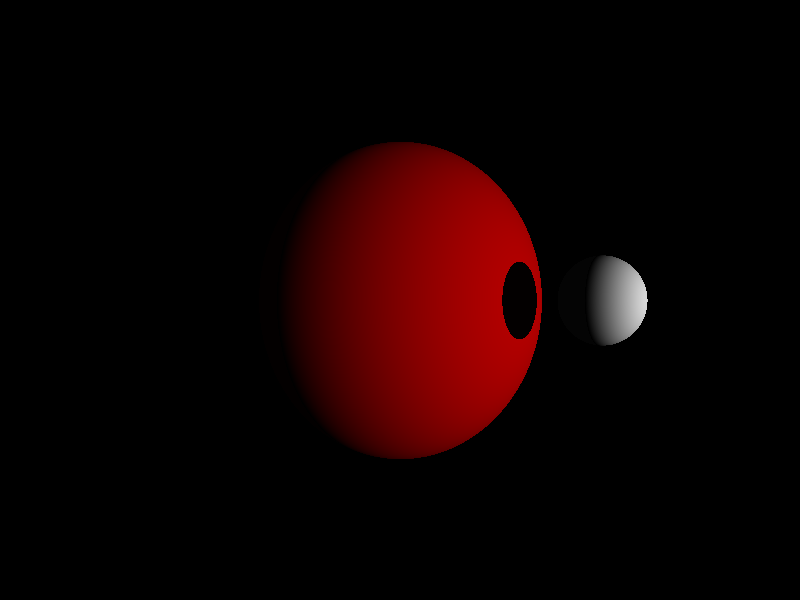
\includegraphics[width=\textwidth, keepaspectratio=true]{../../diary/06.png}
  \caption{Projection de l'ombre \tsl{dure}\ de la sphère grise sur la sphère
  rouge.\label{fig:hardshadow}}
\end{figure}

Pour éviter cet effet, il s'agit d'utiliser des lumières non plus ponctuelles
et discrètes, mais surfacique et continue.

Ainsi, plutôt que d'établir l'appartenance d'un point à une zone d'ombre en
lançant un seul rayon vers la source de lumière nous répétons cette opération
sur toute la surface de la lumière (en utilisant une distribution statistique
de notre choix) et en faisant la moyenne.

\subsection{Exemple}
Une telle technique, permet, au prix d'une perte de performance, d'obtenir des
résultats du type de la \tsl{fig. \ref{fig:softshadows}}.

\begin{figure}[h]
  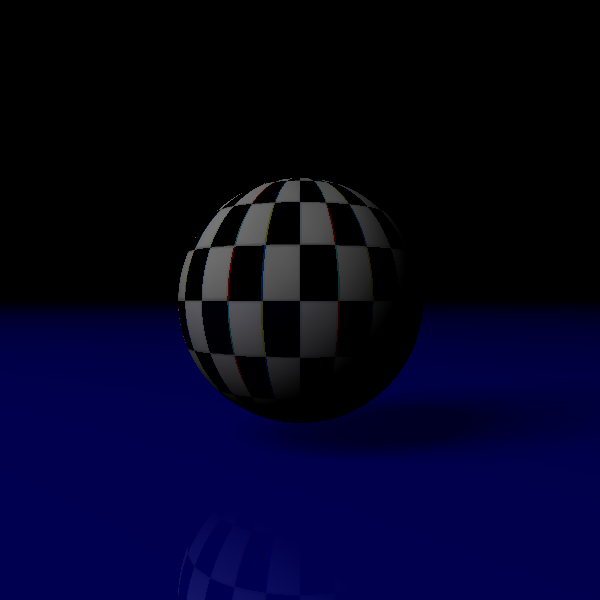
\includegraphics[width=\textwidth, keepaspectratio=true]{../../diary/21.png}
  \caption{Un exemple de rendu des ombres douces\label{fig:softshadows}}
\end{figure}

\subsection{Amélioration}
\begin{description}
  \item [Ajout de lumières surfaciques] Pour le moment, la seule lumière
    surfacique qui est implémentée est la lumière plane. Il pourrait être
    pratique de disposer de lumière sphérique par exemple.
\end{description}

\subsection{Bug connu}
Aucun.
